Grundsätzlich werden die Middleware-Headers als Sicherheitsmaßnahmen verwendet. Das heißt es ist schwieriger für Hacker:innen Informationen über die Software herauszufinden. Es gibt einige verschiedene Middleware-Header:

\begin{itemize}
    \item \textbf{Allow-Cors Header}
        \newline
        Cors (Cross-Origin Resource Sharing) wurde als Sicherheitsmethode von Webbrowsern implementiert, um den Zugriff auf Ressourcen von einer anderen Domain einzuschränken. Wenn ein Client eine Anfrage an einen Server sendet, kann der Server durch Hinzufügen eines speziellen Headers, namens Access-Control-Allow-Origin bestimmen, welche Domains Zugriff auf seine Ressourcen haben dürfen. Sollte die anfragende Domain nicht in der erlaubten Liste enthalten sein, wird der Browser die Anfrage blockieren.

        Im Fall dieser Diplomarbeit wurde Cors folgendermaßen verwendet:

\begin{lstlisting}[caption=Verwendung von Cors]
    const cors = require('cors');
    app.use(cors())
\end{lstlisting}
                
\begin{figure}[h]
    \centering
    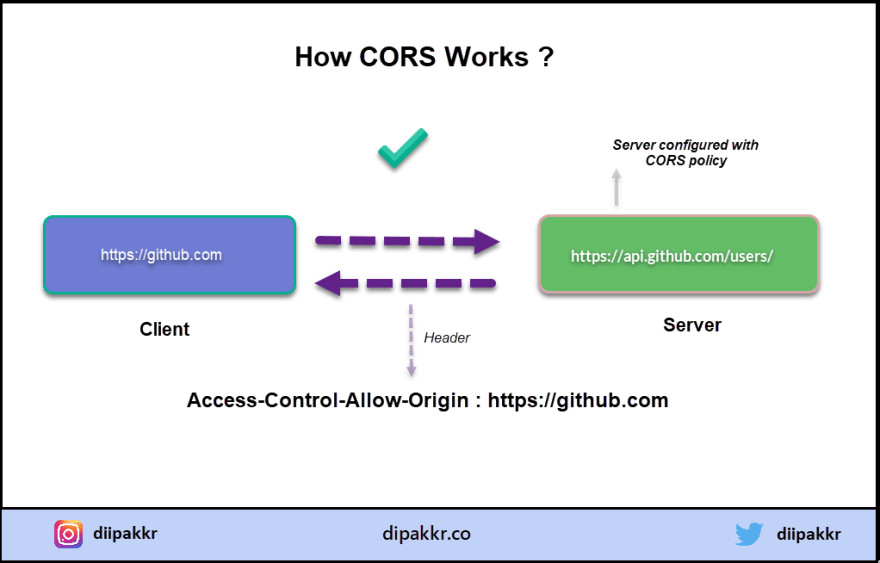
\includegraphics[width=0.5\textwidth]{pics/cors.png}
    \caption{Cors}
    \label{fig:mesh1}
    \cite{cors_grafik}
\end{figure}

        \cite{Cors}
    \item \textbf{Compression Header}
        \newline
        Wenn eine API eine Response mit einer sehr großen Datenmenge von sich gibt, kann hier der Compression Header verwendet werden, um die Antworten vom Server zu schmälern. Wenn eine HTTP-Anfrage mit dem Header "Accept-Encoding" gesendet wird, ermöglicht dies dem Server, die Antwort im unterstützten Format komprimiert zu senden.

        Simulation einer Server Response von (~550k bytes) und Einbindung des Compression-Headers:
            \begin{lstlisting}
                const express = require('express');
                const app = express();
                const compression = require('compression');
                app.use(compression());
                app.get('/', function(req, res) {
                    res.send('hello world'.repeat(50000));
                });
                app.listen(3000, function(err) {
                    if (err) console.log(err);
                    console.log("Server listening on PORT 3000");
                });
            \end{lstlisting}
    \item \textbf{Helmet}
        \newline
        Helmet dient zur Sicherung der HTTP Headers. Es ist eine Sammlung von insgesamt 12 Node-Modulen. Jedes einzelne davon bietet Konfigurationsoptionen zur Sicherung der verschiedenen HTTP-Header. Hier ist eine Liste der verschiedene Node-Module welche gesichert werden.
        \begin{itemize}
            \item Content-Security-Policy
            \item Cross-Origin-Embedder-Policy
            \item Cross-Origin-Opener-Policy
            \item Cross-Origin-Resource-Policy
            \item Origin-Agent-Cluster
            \item Referrer-Policy
            \item Strict-Transport-Security
            \item X-Content-Type-Options
            \item X-DNS-Prefetch-Control
            \item X-Download-Options
            \item X-Frame-Options
            \item X-Permitted-Cross-Domain-Policies
            \item X-Powered-By
            \item X-XSS-Protection
        \end{itemize}
        \newpage
        Die Einbindung von Helmet erfolgte folgendermaßen:

            \begin{lstlisting}[caption=Verwendung von Helmet]
                const express = require('express');
                const app = express();
                const helmet = require('helmet')
                app.use(helmet())
            \end{lstlisting}

        \cite{Helmet}
    \item \textbf{No-Cache-Header}
        \newline
        Im Caching Header werden die Caching-Rechtslagen für Client-Anfragen und Server Antworten festgelegt. Die Caching-Richtlinien bestimmen, wie die Ressource zwischengespeichert wird, wo sie zwischengespeichert wird und für welche Dauer sie zwischengespeichert werden kann, bevor sie abläuft. Der Cache Header besitzt ein "Expires" Property, dieses gibt an, nach welchem Datum die Anfrage als abgelaufen gilt. Um höchste Genauigkeit zu gewährleisten, kann der Parameter "max-age" in Sekunden angegeben werden.

        In dieser Diplomarbeit wurde der No-Cache-Header folgendermaßen umgesetzt:

        \begin{lstlisting}
        module.exports = (req, res, next) => {
            res.header({
            'Cache-Control': 'public, max-age=0',
            Expires: new Date(Date.now()).toUTCString()
        })
        next()
        }
        \end{lstlisting}

        In diesem Fall wird das Property "Expires" auf das aktuelle Datum gesetzt, somit läuft der Cache im selben Moment ab und es wird nichts gecached.


        \cite{No_Cache_Header}
        
\end{itemize}